\documentclass{article}


% if you need to pass options to natbib, use, e.g.:
%     \PassOptionsToPackage{numbers, compress}{natbib}
% before loading neurips_2022


% ready for submission
\usepackage[preprint]{neurips_2022}


% to compile a preprint version, e.g., for submission to arXiv, add the
% [preprint] option:
%     \usepackage[preprint]{neurips_2022}


% to compile a camera-ready version, add the [final] option, e.g.:
%     \usepackage[final]{neurips_2022}


% to avoid loading the natbib package, add option nonatbib:
%    \usepackage[nonatbib]{neurips_2022}


\usepackage[utf8]{inputenc} % allow utf-8 input
\usepackage[T1]{fontenc}    % use 8-bit T1 fonts
\usepackage{hyperref}       % hyperlinks
\usepackage{url}            % simple URL typesetting
\usepackage{booktabs}       % professional-quality tables
\usepackage{amsfonts}       % blackboard math symbols
\usepackage{nicefrac}       % compact symbols for 1/2, etc.
\usepackage{microtype}      % microtypography
\usepackage{xcolor}         % colors
\usepackage{graphicx}
\usepackage{csvsimple}

\usepackage{float}
\usepackage{makecell}




\title{Intention Classification with Pretrained Language Models}


% The \author macro works with any number of authors. There are two commands
% used to separate the names and addresses of multiple authors: \And and \AND.
%
% Using \And between authors leaves it to LaTeX to determine where to break the
% lines. Using \AND forces a line break at that point. So, if LaTeX puts 3 of 4
% authors names on the first line, and the last on the second line, try using
% \AND instead of \And before the third author name.

\author{%
    Xiyan Shao \\
    UCSD \\
    \texttt{x3shao@ucsd.edu} \\
    \And
    Yunxiang Chi \\
    UCSD \\
    \texttt{yuchi@ucsd.edu} \\
    \And
    Zelong Wang\\
    UCSD \\
    \texttt{zew013@ucsd.edu} \\
    \And
    Zhaoyu Zhang\\
    UCSD \\
    \texttt{zhz057@ucsd.edu} \\
}

\begin{document}

    \maketitle

    \begin{abstract}
    Intention classification is an important task in building dialog systems and AI assistants.
    In this paper, we implemented models for intention classification with pretrained language models.
    For fine tuning, we applied LLDR and SWA to better fine tuning, and contrastive learning to improve the performance.
    Our best model achieved a achieve an 84\% accuracy on the intent classification task on the Amazon dataset.

    \end{abstract}


    \section{Introduction}

    Intention classification is an important task in building dialog systems and AI assistants.
    It is the first step in a dialog system to understand the user's utterance and decide what to do next.
    In this work, we implement novel models that approaches intention classification with the power of pretrained language models.
    We use the pretrained language models to extract the contextualized representations of the utterances and then use the representations to train a classifier.
    We also applied various optimization techniques as well as contrastive learning in an attempt to improve the performance of the models.
    Specifically, we implemented LLDR and SWA to help with fine-tuning the pretrained language models.
    We also implemented the strategies of contrastive learning described in \cite{gaoSimCSESimpleContrastive2022} and \cite{khoslaSupervisedContrastiveLearning2021} to improve the performance of the models.
    As the result, we were able to achieve an 84\% accuracy on the intent classification task on the Amazon dataset.


    \section{Related Work}

    Intention classification with pretrained language models has been studied in \cite{chenBERTJointIntent2019} and \cite{larsonEvaluationDatasetIntent2019}
    and \cite{wuTODBERTPretrainedNatural2020}.
    The contrastive learning losses have been studied in \cite{khoslaSupervisedContrastiveLearning2021} for CV tasks and \cite{gaoSimCSESimpleContrastive2022} for NLP tasks.
    The LLDR and SWA optimization techniques are studied in \cite{changAdvancedTechniquesFinetuning2021}.
    We also heavily relied on Gary's lecture slides and PyTorch's documentation to implement the models.


    \section{Experiments}

    \subsection{Baseline Model}

%    (a) It has at least 3 subsections for baseline/custom/contrastive learning. Each of the subsection should
%start with the final experimental settings you decide that we do not specify, including parameters of
%the library functions (except for defaults), hyperparameters you choose etc. These experimental setting
%should correspond to your best results.

%    (b) Summarize and document how you reach these experimental settings in each of the subsections. Select
%some milestone improvements (not all the things you have tried) and document them in the report. For
%example,
%“We start with setting A (with learning rate=<this>, ...), the results are <this>. We figure out this
%result is limited by learning rate because... After fixing the learning rate, it can reach <this> perfor-
%mance. We further figure out the new result is limited by..., because... We fixed it and the performance
%becomes... Finally, it reaches the reported results.”

    We implemented the baseline model and trained the final model with the following hyperparameters:

    \begin{table}[H]
        \centering
        \begin{tabular}{ll}
            \toprule
            \textbf{Hyperparameter} & \textbf{Value} \\
            \midrule
            Scheduler Type          & Constant       \\
            Warmup Epochs           & 0              \\
            Learning Rate           & 0.0001         \\
            Adam Epsilon            & 1e-8           \\
            $n$ Epochs              & 10             \\
            Batch Size              & 256            \\
            \bottomrule
        \end{tabular}
        \caption{Hyperparameters of the final model for baseline}
        \label{tab:hyps_baseline}
    \end{table}

    We started with a learning rate of 0.01 and applied a \texttt{StepLR} scheduler but was not able to achieve a reasonable
    accuracy (final accuracy was approximately 0.06).
    We figured that this is because the decay rate of the scheduler is too high.
    Hence, we decided to use a simple constant learning rate scheduler and experimented with different learning rates.
    We found that a learning rate of 0.0001 is the best choice for our model.
    We also experimented with different values of Adam epsilon and found that 1e-8 is the best choice.
    Another hyperparameter that we tuned is the batch size.
    We found that a batch size of 256 outperformed other batch sizes and was more efficient in terms of training time.
    Finally, we decided the set of hyperparameters as described in Table~\ref{tab:hyps_baseline}.
    The final accuracy was 0.84.

    \subsection{Custom Model}
    Based on the results of baseline, we continue to use some common hyperparameters like 0.0001 learning rate, constant scheduler type, 1e-8 Adam Epsilon, and 256 batch size.
    \subsubsection{Layer-wise Learning Rate Decay}
    For second choice, we chose to implement Layer-wise Learning Rate Decay to better fine-tuning the model using the following hyperparameters:

    \begin{table}[H]
        \centering
        \begin{tabular}{ll}
            \toprule
            \textbf{Hyperparameter} & \textbf{Value} \\
            \midrule
            Scheduler Type          & Constant       \\
            Warmup Epochs           & 0              \\
            Head Learning Rate      & 0.00031         \\
            Layer 11 Learning Rate  & 0.0003         \\
            Layer 0 Learning Rate  & 0.0.000085         \\
            Embedding Learning Rate  & 0.0.000076        \\
            Layer-wise Learning Rate Decay  & 0.9    \\
            Adam Epsilon            & 1e-8           \\
            $n$ Epochs              & 10             \\
            Batch Size              & 256            \\
            Dropout                 & 0.9            \\
            \bottomrule
        \end{tabular}
        \caption{Hyperparameters of the Layer-wise Learning Rate Decay Model}
        \label{tab:hyps_LLRD}
    \end{table}
    First, after building the Layer-wise Learning Rate Decay (LLRD), we used the exact learning rate and learning rate decay as introduced in "Advanced Techniques for Fine-tuning Transformers", which leads to a very poor result. We figured that the learning rate suitable in their model might not be a reasonable one for us.\\
    Then, we following the conclusions from the Baseline model above using mostly the same hyperparameters. We start from using a head learning rate of 0.00014, Layer 11 Learning Rate of 0.00013 and learning rate decay of 0.9 for each layer. The resulting accuracy raised to around 0.6. We also tried a decay of 0.95, but the accuracy is not improving. \\
    We further choose a wider learning rate range. We set head learning rate to 0.00031, Layer 11 Learning Rate to 0.0003, and learning rate decay to 0.9. The resulting accuracy raised to around 0.62. Finally, it reaches the reported results\\

    \subsubsection{Stochastic Weight Averaging(SWA)}
    For second choice, we chose to implement Stochastic Weight Averaging(SWA) to better fine-tuning the model using the following hyperparameters:

    python main.py --n-epochs 10 --do-train --task custom --reinit_n_layers 5 --swa-start 5 --scheduler-type constant
    \begin{table}[H]
        \centering
        \begin{tabular}{ll}
            \toprule
            \textbf{Hyperparameter} & \textbf{Value} \\
            \midrule
            Scheduler Type          & Constant       \\
            Learning Rate           & 0.0001         \\
            Adam Epsilon            & 1e-8           \\
            $n$ Epochs              & 15             \\
            Batch Size              & 256            \\
            SWA Start Step          & 6              \\
            SWA learning rate       & 1e-4           \\
            \bottomrule
        \end{tabular}
        \caption{Hyperparameters of the final model for custom_2 SWA}
        \label{tab:hyps_swa}
    \end{table}

    We firstly set up the SWA start step as 3, SWA learning rate as 2e-6, and epochs as 256.
    For SWA start step, we noticed that when the model trained at the SWA start step, its accuracy increase less than that of the past epoches.
    We believed the learning rate will be 2e-6 and remain constant after the SWA start step, which might be the reason for unreasonable accuracy, which is 0.44.
    Thus, we tested with different SWA learning rates: 1e-6 and 3e-6.
    It turned out that both smaller swa learning rate won't help, but changing the swa learning rate to a larger one seems help a lot, so we decided to experiment with more larger swa learning rate.
    After multiple experiments, we found 1e-4 is the best choice for swa learning rate.
    Then, for start step, 6 is the best choice from experiments.
    Since the start step for SWA should be set to a later epoch, we may need to train more epoches to display the effects of SWA.
    After some experiments, 15 epoches is the best choice that can better prevent overfits.
    The final accuracy was 0.845.


    \subsection{Contrasive Learning}
    We implemented the contrastive learning model (both SupCon and SimCLS) and trained the final models with the following hyperparameters:

    \begin{table}[H]
        \centering
        \begin{tabular}{ll}
            \toprule
            \textbf{Hyperparameter} & \textbf{Value} \\
            \midrule
            Scheduler Type          & Constant       \\
            Warmup Epochs           & 0              \\
            Learning Rate           & 0.0001         \\
            Adam Epsilon            & 1e-8           \\
            $n$ Epochs              & 10             \\
            Batch Size              & 256            \\
            Dropout                 & 0.2            \\
            \bottomrule
        \end{tabular}
        \caption{Hyperparameters of the final contrastive learning models}
        \label{tab:hyps_contrastive}
    \end{table}

    We started with a linearly decaying learning rate of 0.0005, warmup epochs of 2, and drop rate of 0.9.
    Nevertheless, the final embedding plot did not present clear clusters, and the loss only decreased by around 15\%.
    Then, we thought that maybe the learning rate is too high, so we decreased it to 0.0001 and used a constant learning rate
    scheduler as in part 1, yet this change did not help with performance.
    We also tested other hyperparameters including batch size, enabling LLDR, and using a different optimizer.
    None of the changes
    improved the final embedding plot or the loss.
    Finally, we decided to decrease the dropout rate to 0.2 and the training loss improved significantly.
    This is because with too a very high dropout rate, we are effectively applying a strong corruption to the input as the
    augmentation, which is not helpful for the model to learn the similarity representation.
    By making the dropout rate smaller, the augmentation was more subtle and the final embedding plot presented well-demarcated
    clusters.


    \section{Discussion}
    \textbf{Q1:} If we do not fine-tune the model, what is your expected test accuracy (1 sentence)? Why (1 sentence)?\\
    \textbf{A1:} We expected it have smaller accuracy than the model after fine tuning. Because fine-tuning will update additional parameters and pretrained BERT parameters to fit training data of downstream tasks.

    \begin{tabular}{|c|c|c|c|}
        \hline $\exp$ idx & $\exp$                      & loss & accuracy \\
        \hline 1          & Test set before fine-tuning &   3.69   &     0.059     \\
        2                 & Test set after fine-tuning  &  0.54    &    0.84     \\
        \hline
    \end{tabular}

    \textbf{Q2:} Do results match your expectation(1 sentence)? Why or why not (1-2 sentences)?\\
    \textbf{A2:} Yes, it matches our expectation. Because fine-tuning will update additional parameters and pretrained BERT parameters to fit training data of downstream tasks.

    \textbf{Q3:} What could you do to further improve the performance (1 sentence)?\\
    \textbf{A3:} We can apply more advanced optimization techniques such as non-constant learning rate scheduling, weight decay, early stopping, LLDR, SWA, and so on.

    \textbf{Q4:} Which techniques did you choose and why? (1 sentence)?\\
    \textbf{A4:} Our first technique is Layer-wise Learning Rate Decay, and the second one is Stochastic Weight Averaging(SWA).
    We choose Layer-wise Learning Rate Decay (LLRD) because different layers in the Transformer model might be responsible for different jobs.
    For example, as mentioned in "Advanced Techniques for Fine-tuning Transformers", bottom layers often encode more common, general, and broad-based information,
    while the top layer closer to the output encodes information more localized and specific to the task on hand such as our classification of user instruction texts.
    The reason of choosing SWA is that we believe it can improve the stability of training and final testing accuracies.

    \textbf{Q5:} What do you expect for the results of the individual technique vs. the two techniques combined? (1 sentence)?\\
    \textbf{A5:} We expect combining two techniques will show better performance than that of only one individual technique.

    \begin{tabular}{|c|c|c|c|}
        \hline $\exp$ idx & $\exp$                      & loss & accuracy \\
        \hline 1          & Test set with 1st technique &  1.63    &    0.62     \\
        2                 & Test set with 2nd technique &  0.30    &    0.85     \\
        3                 & Test set with 2 techniques  &  1.63    &    0.62     \\
        \hline
    \end{tabular}

    \textbf{Q6:} Do results match your expectation(1 sentence)? Why or why not (1-2 sentences)?\\
    \textbf{A6:} No, they didn't match. We believe the reason is that when we combined lldr and SWA, the lldr won't be able to provide a good learning rate to SWA. Therefore, SWA will malfunction after the starting step.
    Thus, using SWA individually will display better performance then combining them together.

    \textbf{Q7:} What could you do to further improve the performance (1 sentence)?\\
    \textbf{A7:} For lldr, we could increase the number of searched space for each layer, and we can also set different width decay for different layers.
    For swa, we could do more experiment and try to get a better swa learning rate and better swa start step, which won't negatively affect the performance while enhancing the stability.

    \textbf{Q8:} Compare the SimCLR with SupContrast. What are the similarities and differences?\\
    \textbf{A8:} Both SupContrast and SimCSE  exploits contrastive loss which aims to have similar embedding for same class and dissimilar embeddings for different classes.
    SimCSE will make different augmentations of the same class have the similar embeddings and it will recognize different pictures of the same class as different. SupContrast will use labels during the loss calculation and won't consider different pictures from different classes different.

    \textbf{Q9:} How does SimCSE apply dropout to achieve data augmentation for NLP tasks?\\
    \textbf{A9:} SimCSE uses independently sampled dropout masks on sentences with specified dropout probabilities to drop noise.

    \textbf{Q10:} If we do not fine-tune the model, how do the embeddings of the [CLS] tokens look like (1 sentence)?\\
    \textbf{A10:} We expected that the distribution of the embeddings from different classes will be more random and each cluster are more likely to contain dissimilar classes.


    \textbf{Q11:} What can be the differences between the the embeddings of the [CLS] tokens fine-tuned through cross-entropy, SupContrast, and SimCLR (1-2 sentences)?\\
    \textbf{A11:} We expected that cross-entropy will be more randomly distributed; SimCLR will have clusters but dissimilar classes may come into the same cluster and same classes will go to different clusters; SupContrast will the embeddings in clusters and each cluster contains similar classes.

    \textbf{Q12:} Do the results match your expectation(1 sentence)? Why or why not (1-2 sentences)?\\
    \textbf{A12:} Results of the SimCLR and SupCon models assligned with our expectations, but the UMAP of of embeddings using cross-entropy loss differed from our conjecture. 
    We think this is because cross entropy loss punishes any difference from the target, that makes the different augmentations of the same graph mapped together, but different picture from the same or similar classes were mapped to different locations.
    We suspect that the SimCLR have a relative random scatter of embeddings was because SimCLR is unsupervised and is slow at learning. 

    \begin{figure}[H]
        \begin{minipage}[b]{0.33\linewidth}
            \centering
            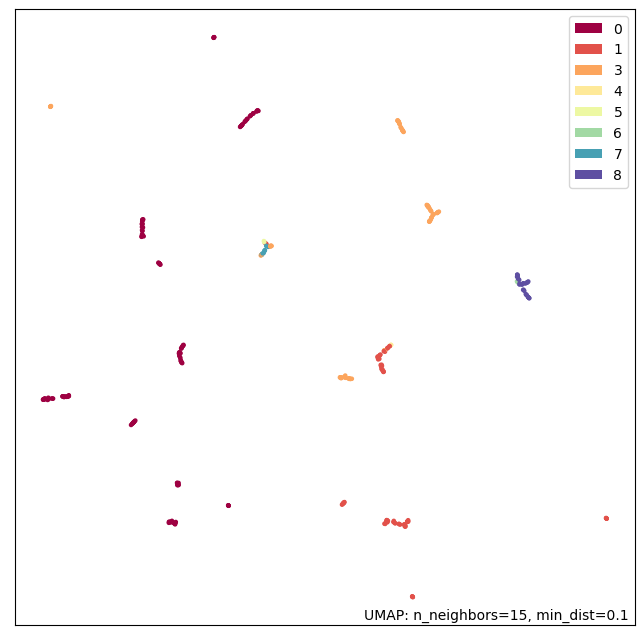
\includegraphics[width=\textwidth]{../results/baseline_umap.png}
            \caption{CE Loss embeddings}
            \label{fig:figure 1.1}
        \end{minipage}
%        \hspace{0.2cm}
        \begin{minipage}[b]{0.33\linewidth}
            \centering
            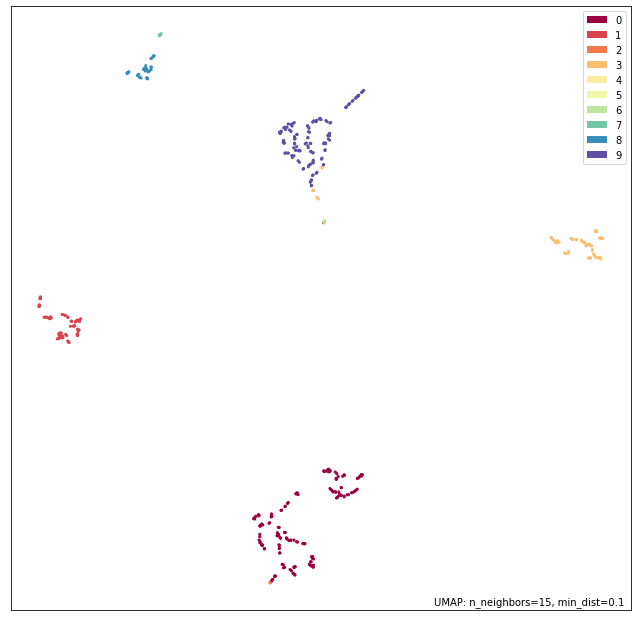
\includegraphics[width=\textwidth]{../results/supcon_256.png}
            \caption{SupCon embeddings}
            \label{fig:figure 1.2}
        \end{minipage}
%        \hspace{0.2cm}
        \begin{minipage}[b]{0.33\linewidth}
            \centering
            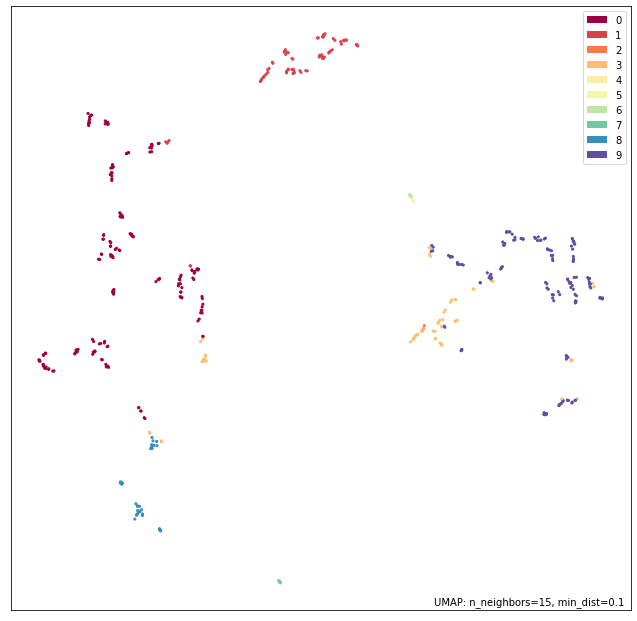
\includegraphics[width=\textwidth]{../results/simclr_64.png}
            \caption{SimCLR embeddings}
            \label{fig:figure 1.3}
        \end{minipage}

    \end{figure}

    

    \textbf{Q13:} What could you do to further improve the performance (1 sentence)?\\
    \textbf{A13:} We suspected that using another MLP layer of pooling or other methods of augmentation might increase the performance.

    Then we also experimented with different batch sizes on SupCon model. We tried batch size of 64, 128, and 256. 
    Even though batch size doesn't influence the clustering of the embeddings a lot, when the data size is greater, the data points of the similar classes gathered closer and there were fewer datapoints went to the wrong cluster.
    \begin{figure}[H]
        \begin{minipage}[b]{0.33\linewidth}
            \centering
            \includegraphics[width=\textwidth]{../results/supcon_64.png}
            \caption{SupCon bacth size 64}
            \label{fig:figure 2.1}
        \end{minipage}
%        \hspace{0.2cm}
        \begin{minipage}[b]{0.33\linewidth}
            \centering
            \includegraphics[width=\textwidth]{../results/supcon_128.png}
            \caption{SupCon bacth size 128}
            \label{fig:figure 2.2}
        \end{minipage}
%        \hspace{0.2cm}
        \begin{minipage}[b]{0.33\linewidth}
            \centering
            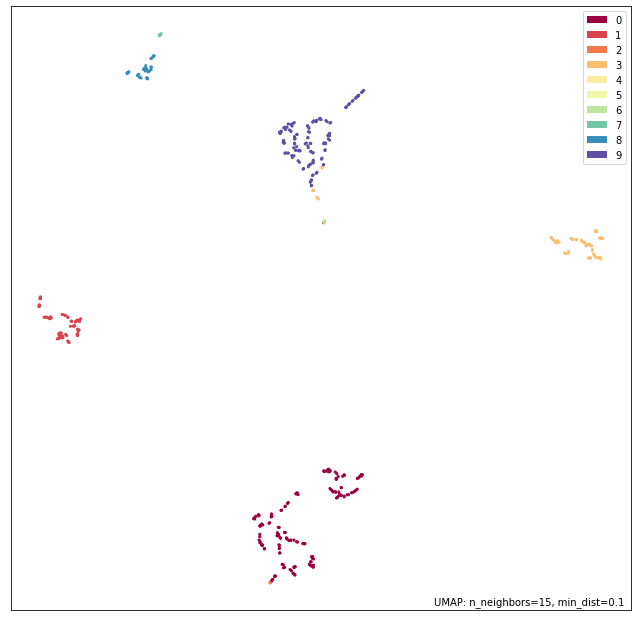
\includegraphics[width=\textwidth]{../results/supcon_256.png}
            \caption{SupCon bacth size 256}
            \label{fig:figure 2.3}
        \end{minipage}

    \end{figure}

    % description of the contributions of each team member

    \section{Contributions}

    \subsection*{Xiyan Shao}
    \begin{itemize}
        \item Implemented the baseline model and the contrastive loss models.
        \item Implemented the UMAP visualization.
        \item Wrote baseline model and contrastive loss models experiments parts of the report.
        \item Wrote the introduction, related work sections of the report.
    \end{itemize}

    \subsection*{Yunxiang Chi}
    \begin{itemize}
        \item Implemented custom model of one of the custom techniques
        \item Experiment with one technique and combining techniques
        \item Wrote one part of the custom model, including expriment and discussion
        \item Wrote the abstract
    \end{itemize}

    \subsection*{Zelong Wang}
    \begin{itemize}
        \item Implemented the baseline model and one of the custom models
        \item Experimented with fine-tuning techniques
        \item Experimented with UMAP
        \item Wrote parts of the custom model, including experiment and discussion
    \end{itemize}

    \subsection*{Zhaoyu Zhang}
    \begin{itemize}
        \item Worked on main method's contrastive learning part
        \item Trained two models of contrastive learning 
        \item Worked answer discussion questions
        \item Wrote report for the discoveries of contrastive learning
    \end{itemize}

\end{document}
